\documentclass{beamer}
\usepackage[latin1]{inputenc}
\usepackage{times}
\usepackage{tikz}
\usetheme{Luebeck}
%\usecolortheme{albatross}
\usepackage{amsmath,amsfonts,amsthm,amssymb}
\usepackage{setspace}
\usepackage{Tabbing}
\usepackage{fancyhdr}
\usepackage{lastpage}
\usepackage{extramarks}
\usepackage{chngpage}
\usepackage{soul,color}
\usepackage{graphicx,float,wrapfig}
\usepackage{xcolor}
\usepackage{listings}
\usepackage{float}
%\usepackage{subfloat}
\usepackage{subfig}
\usepackage{caption}
\usepackage{enumitem}
\usepackage{algpseudocode}

\definecolor{darkorange}{RGB}{240, 120, 0}
\definecolor{darkgreen}{RGB}{0, 128, 0}

\setbeamercolor{background canvas}{bg=white}
\setbeamercolor{frametitle}{fg=white, bg=darkorange}
\setbeamercolor{normal text}{bg=black,fg=black}
\setbeamercolor{structure}{bg=black, fg=darkorange}


\lstdefinestyle{customc}{
  belowcaptionskip=1\baselineskip,
  breaklines=true,
  frame=L,
  xleftmargin=\parindent,
  language=C,
  showstringspaces=false,
  basicstyle=\footnotesize\ttfamily,
  keywordstyle=\bfseries\color{green!40!black},
  commentstyle=\itshape\color{purple!40!black},
  identifierstyle=\color{blue},
  stringstyle=\color{orange},
}

\definecolor{MidGreen}{HTML}{00AA00}
\definecolor{MidYellow}{HTML}{AAAA00}

\title{Lecture 14: Shape Google: Rigid Shape Statistics}
\date{3/1/2016}
\institute{Chris Tralie, Duke University}
\author{COMPSCI/MATH 290-04}
\begin{document}

\frame{\titlepage}

\begin{frame}{Announcements}
\begin{itemize}[label=$\vartriangleright$]

\item Group Assignment 1 Full Submission Due Tomorrow (Wednesday) 11:55 PM

\item Rank Top 3 Final Project Choices By Friday 3/5 (Groups of 3-4)

\item Attendance Policy Clarification

\item Midterm Next Thursday 3/10

\end{itemize}

\end{frame}

\begin{frame}{Table of Contents}
\begin{itemize}[label=$\blacktriangleright$]
	\item Shape Statistics / Algorithms
\end{itemize}
\begin{itemize}[label=$\vartriangleright$]
	\item Comparing Shape Statistics
\end{itemize}
\begin{itemize}[label=$\vartriangleright$]
	\item Classification / Performance Evaluation
\end{itemize}
\end{frame}


\begin{frame}{Random Sampling By Area}

Goal: Given a shape, return similar shapes in a database

\begin{figure}[t]
	\centering
    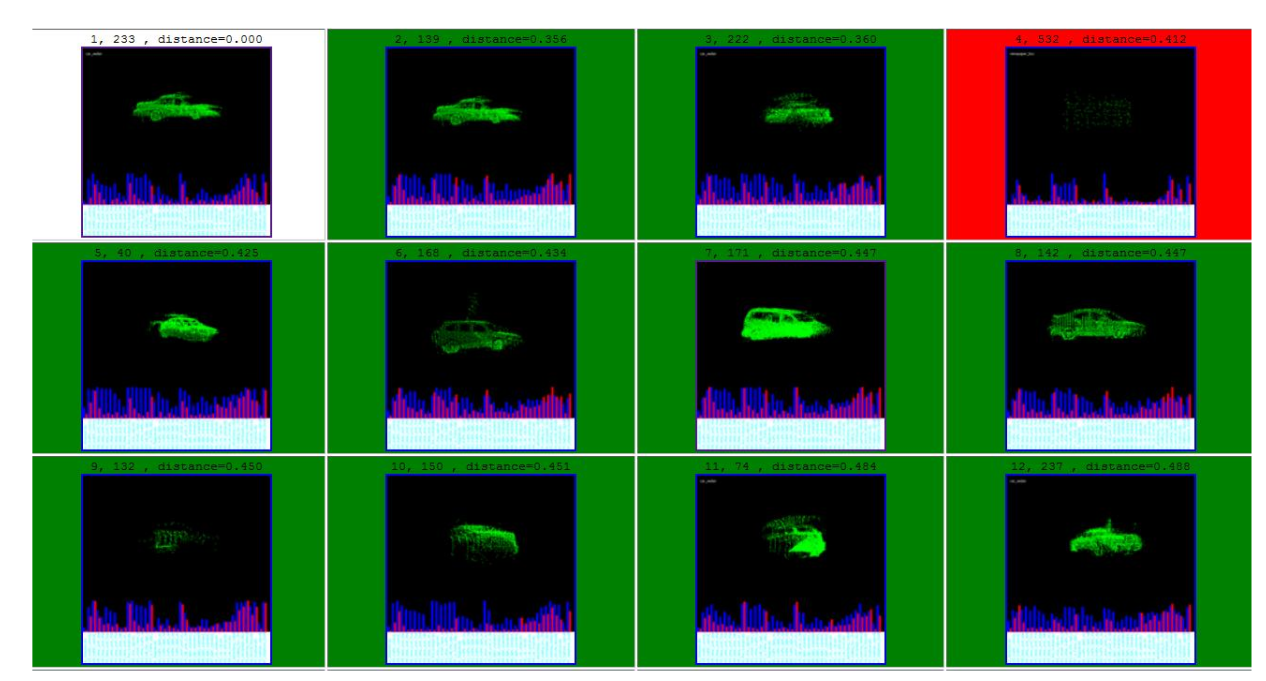
\includegraphics[width=0.8\textwidth]{ShapeGoogle.png}
\end{figure}
\small Tralie 2010

\begin{itemize}[label=$\vartriangleright$]
\item Focus on point clouds
\item Focus on shapes similar under {\em rigid motion}
\end{itemize}

\end{frame}

\begin{frame}{Random Sampling By Area}

\begin{figure}[t]
	\centering
    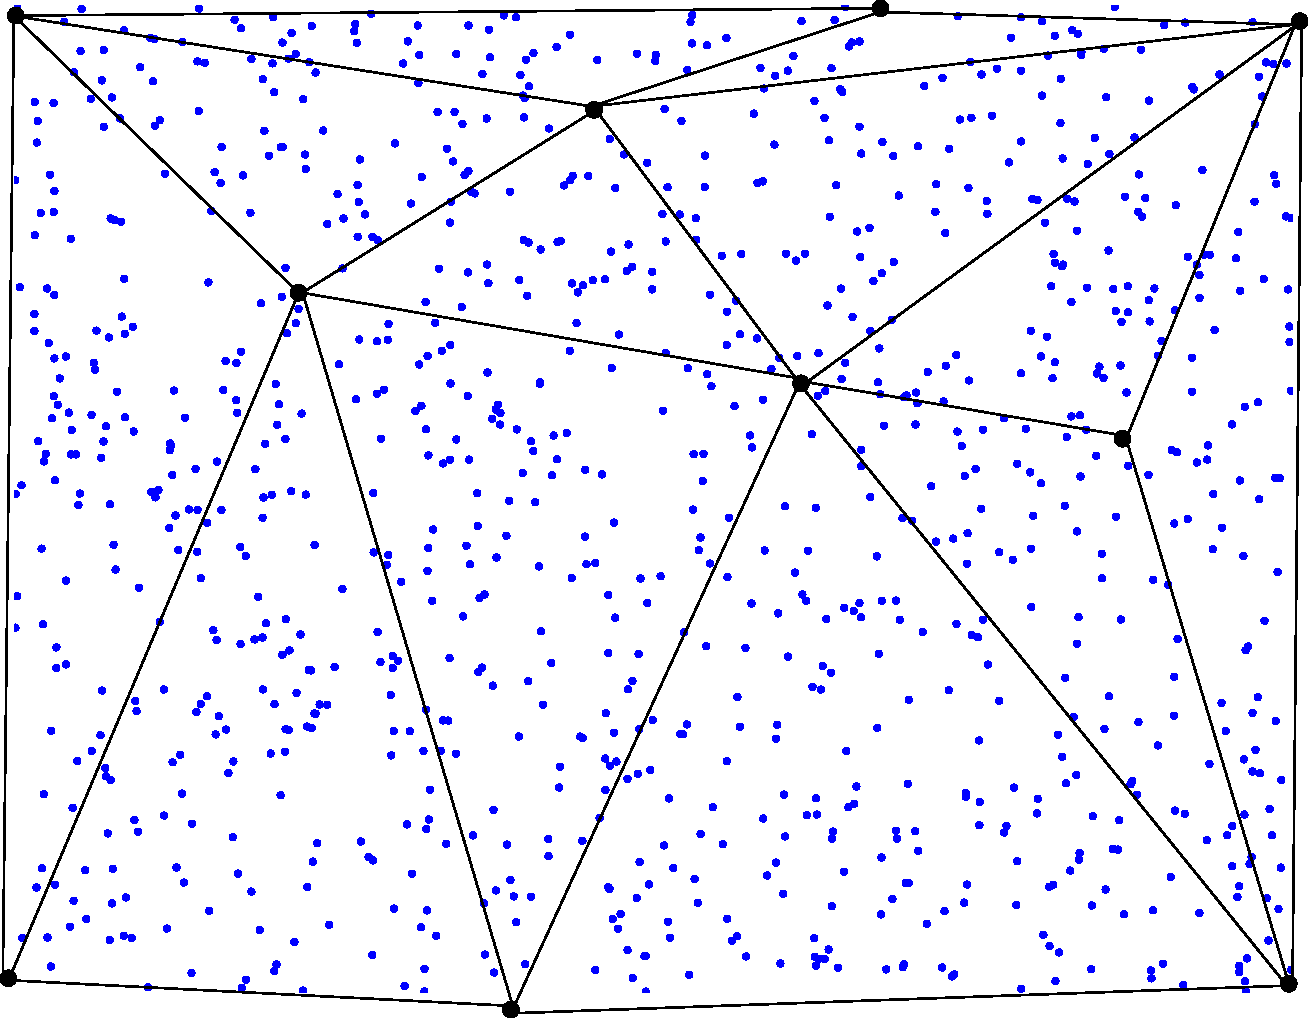
\includegraphics[width=0.8\textwidth]{SampleByArea.pdf}
\end{figure}


\end{frame}


\begin{frame}{Centroid Centering / RMS Scaling}

For a point cloud $\{ \vec{x_i} \}_{i=1}^N$

\begin{itemize}[label=$\vartriangleright$]
\item Subtract off centroid
\item Root mean square scale.  Want

\[ \sqrt{ \frac{1}{N} \sum_{i=1}^N ||\vec{x_i}||^2 } = 1\]

\end{itemize}


\end{frame}

\begin{frame}{Shape Matching Criteria}

\begin{itemize}[label=$\vartriangleright$]
\item Concise To Store

\item Quick to compute


\item Efficient to match


\item Discerning


\item Noise tolerant 


\item {\em Rotation Invariant}

\end{itemize}

\end{frame}

\begin{frame}{Shape Histogram: Shells}

\begin{figure}[t]
	\centering
    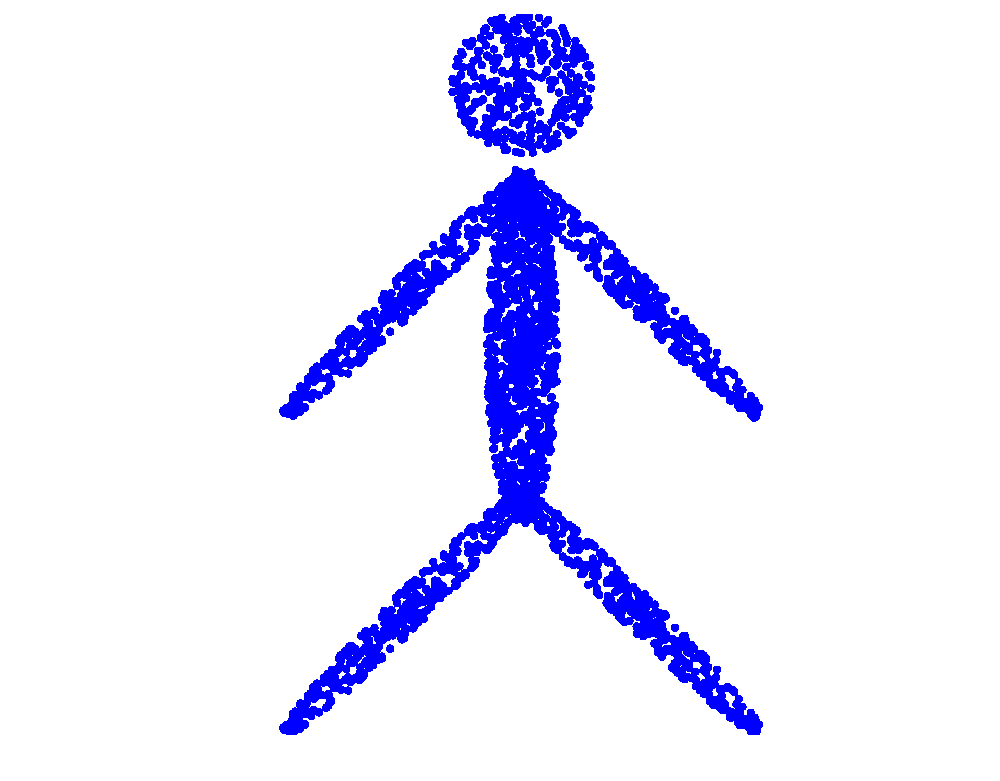
\includegraphics[width=0.7\textwidth]{Person.pdf}
\end{figure}

\end{frame}

\begin{frame}{Shape Histogram: Shells}

\begin{figure}[t]
	\centering
    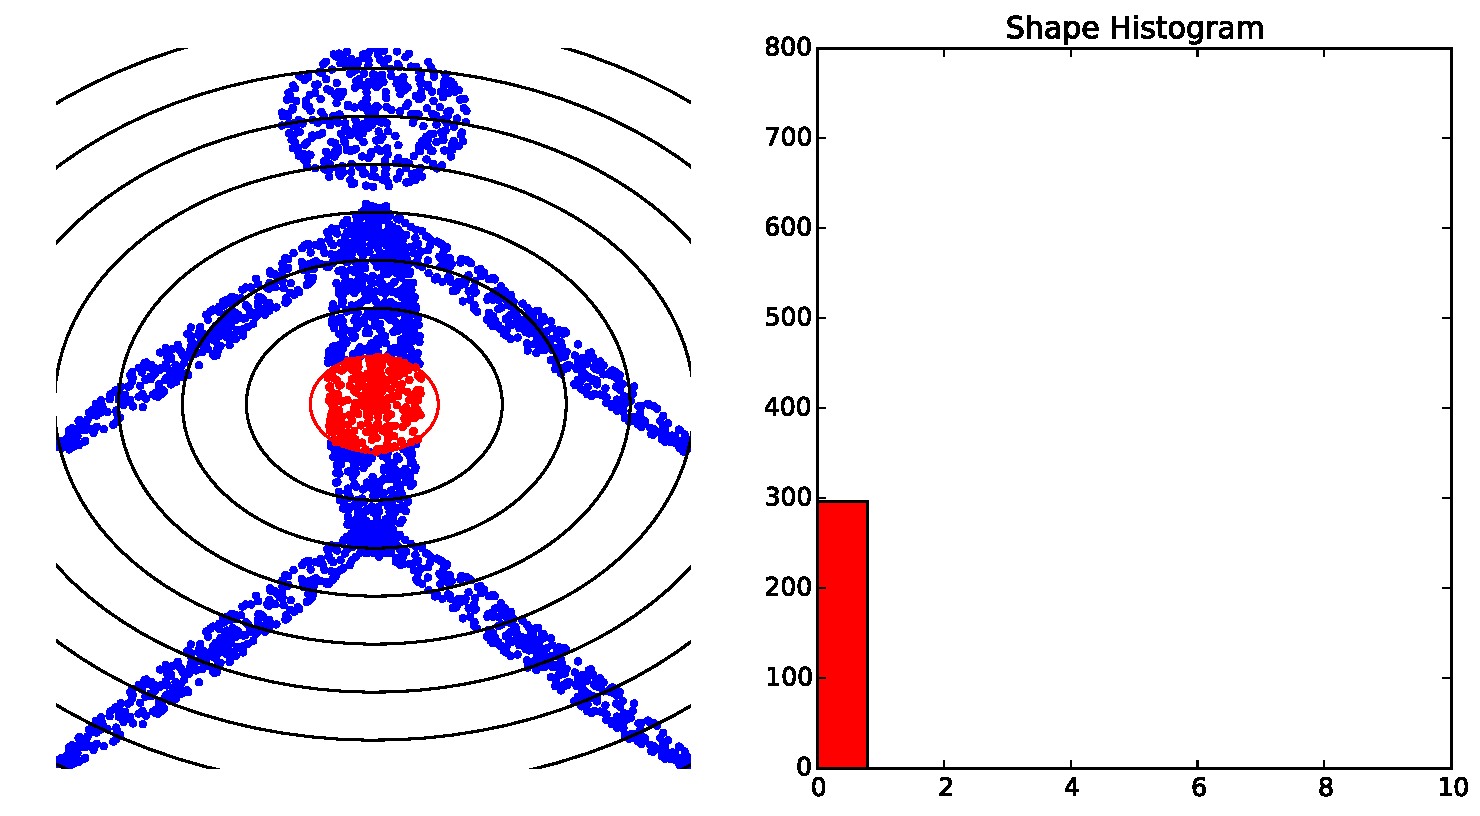
\includegraphics[width=\textwidth]{ShapeHist1.pdf}
\end{figure}

\end{frame}

\begin{frame}{Shape Histogram: Shells}

\begin{figure}[t]
	\centering
    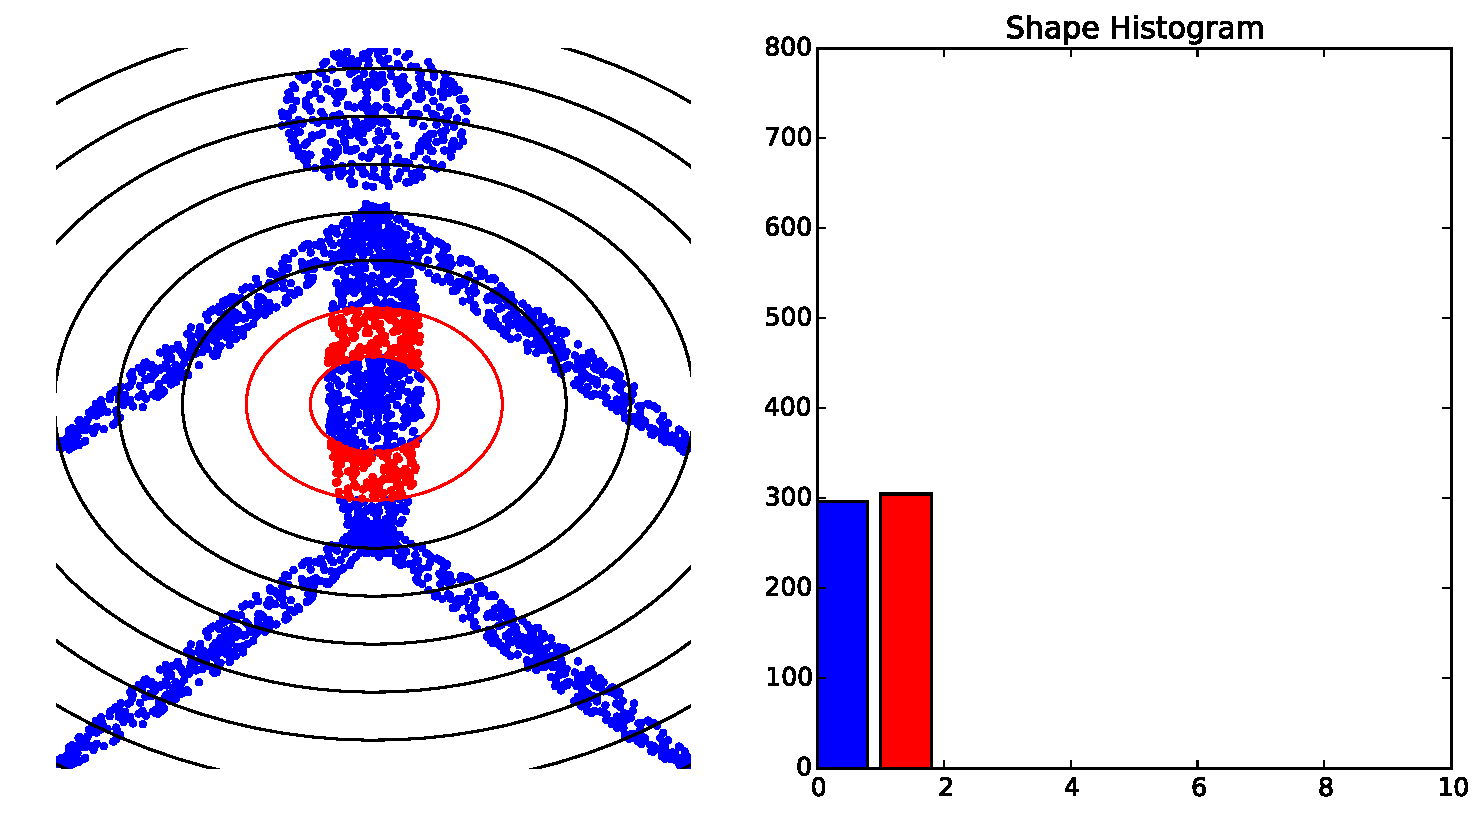
\includegraphics[width=\textwidth]{ShapeHist2.pdf}
\end{figure}

\end{frame}

\begin{frame}{Shape Histogram: Shells}

\begin{figure}[t]
	\centering
    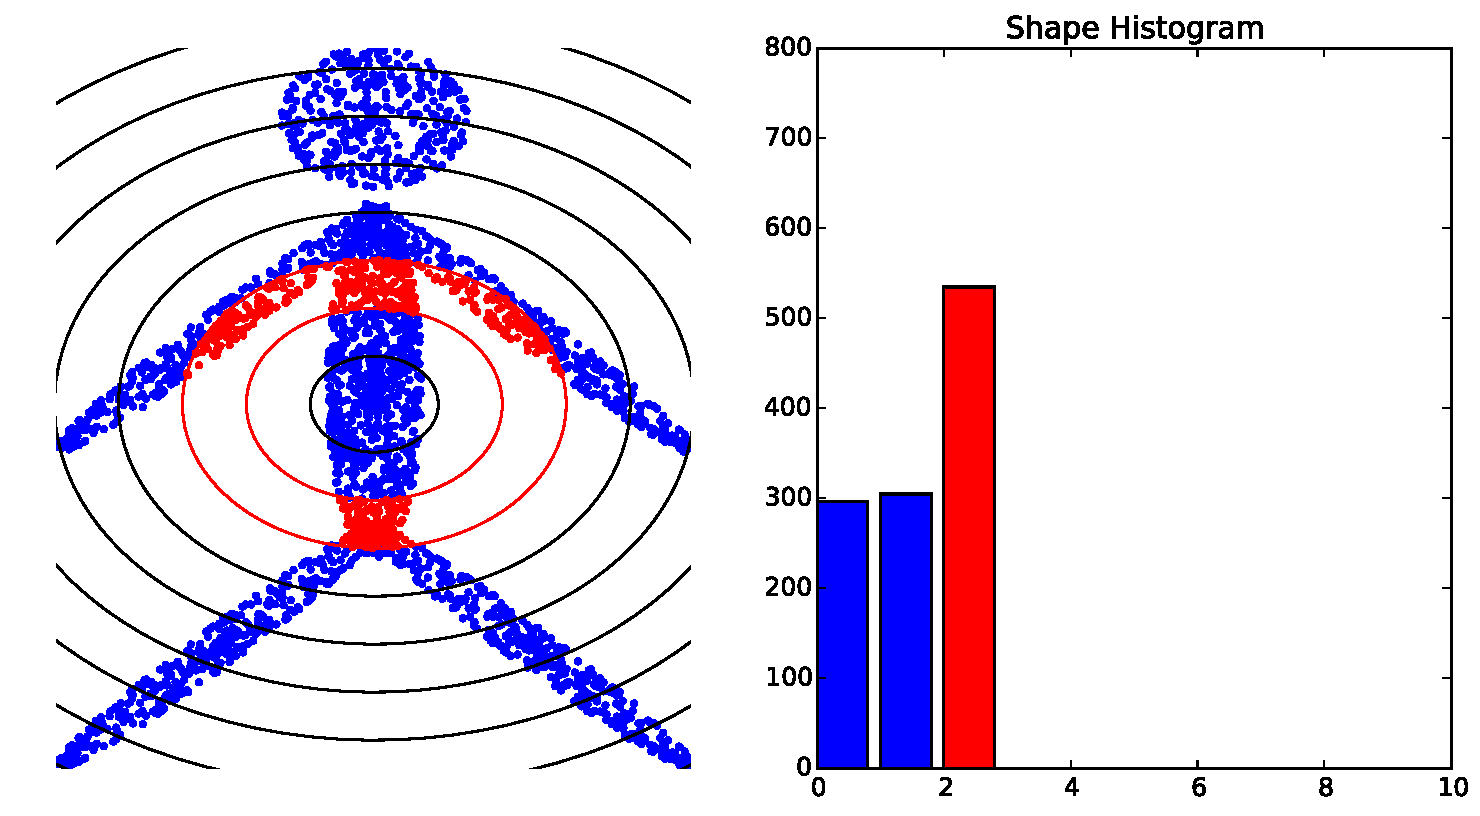
\includegraphics[width=\textwidth]{ShapeHist3.pdf}
\end{figure}

\end{frame}

\begin{frame}{Shape Histogram: Shells}

\begin{figure}[t]
	\centering
    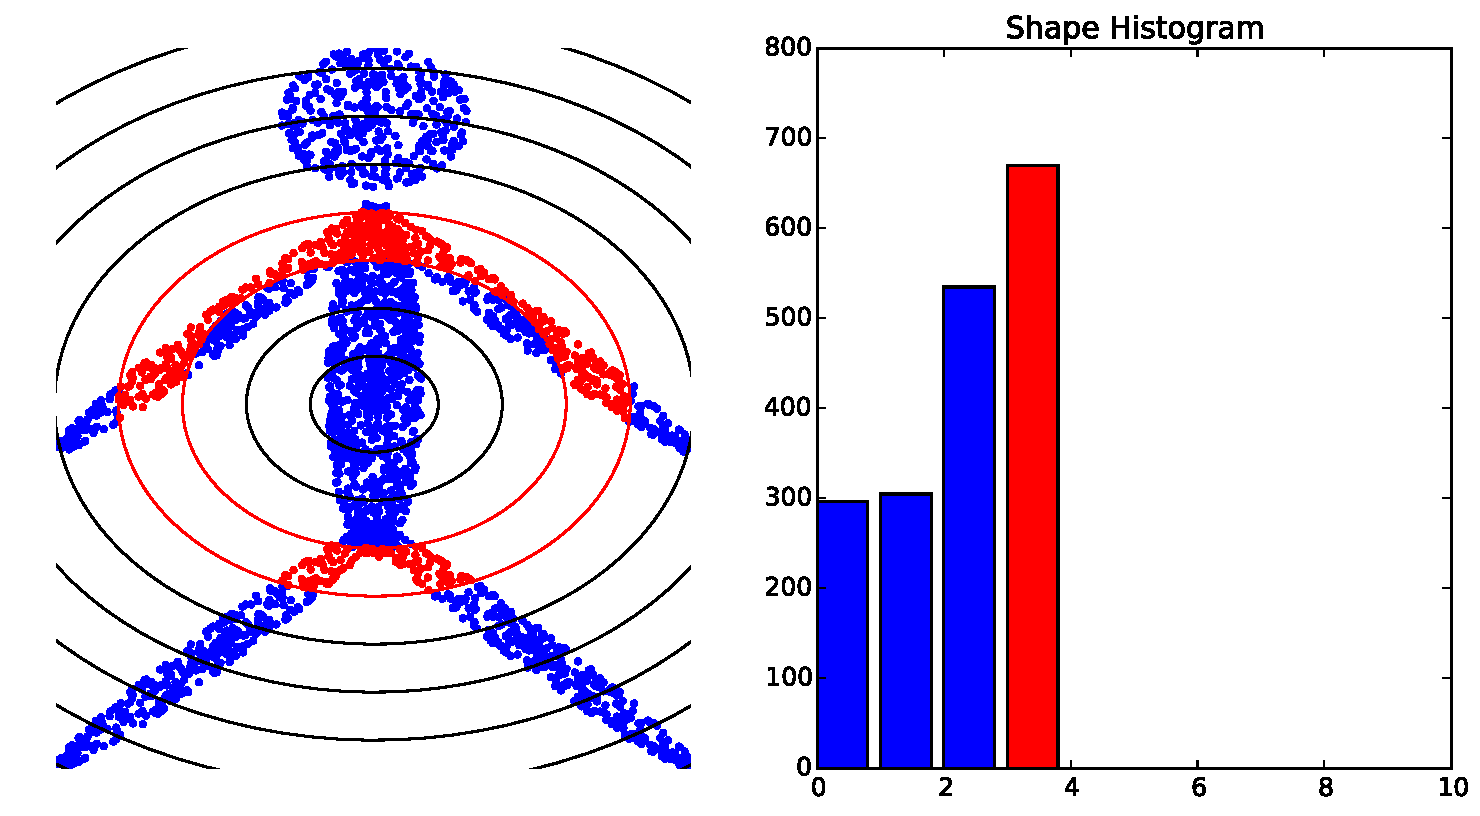
\includegraphics[width=\textwidth]{ShapeHist4.pdf}
\end{figure}

\end{frame}

\begin{frame}{Shape Histogram: Shells}

\begin{figure}[t]
	\centering
    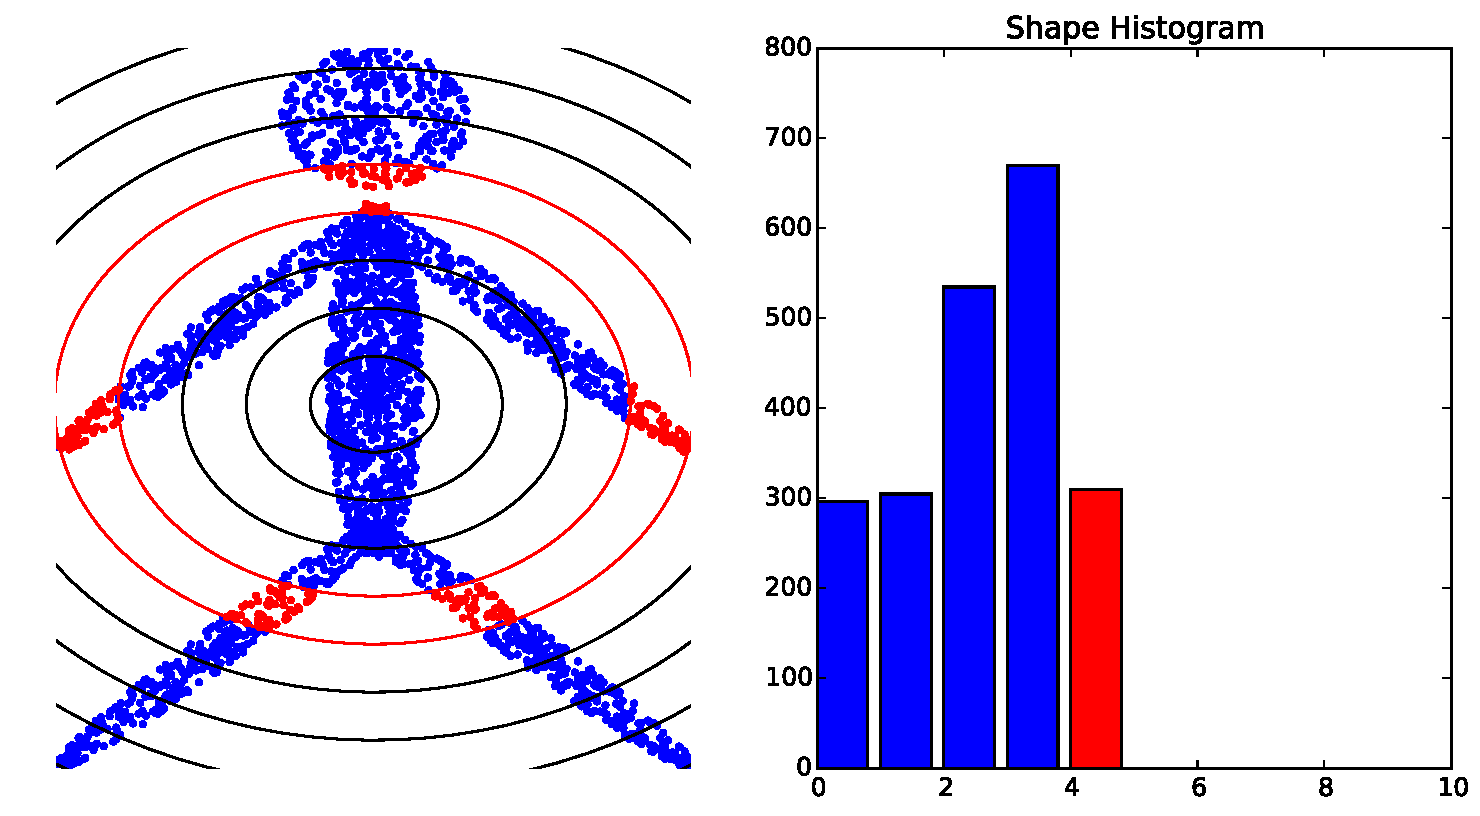
\includegraphics[width=\textwidth]{ShapeHist5.pdf}
\end{figure}

\end{frame}

\begin{frame}{Shape Histogram: Shells}

\begin{figure}[t]
	\centering
    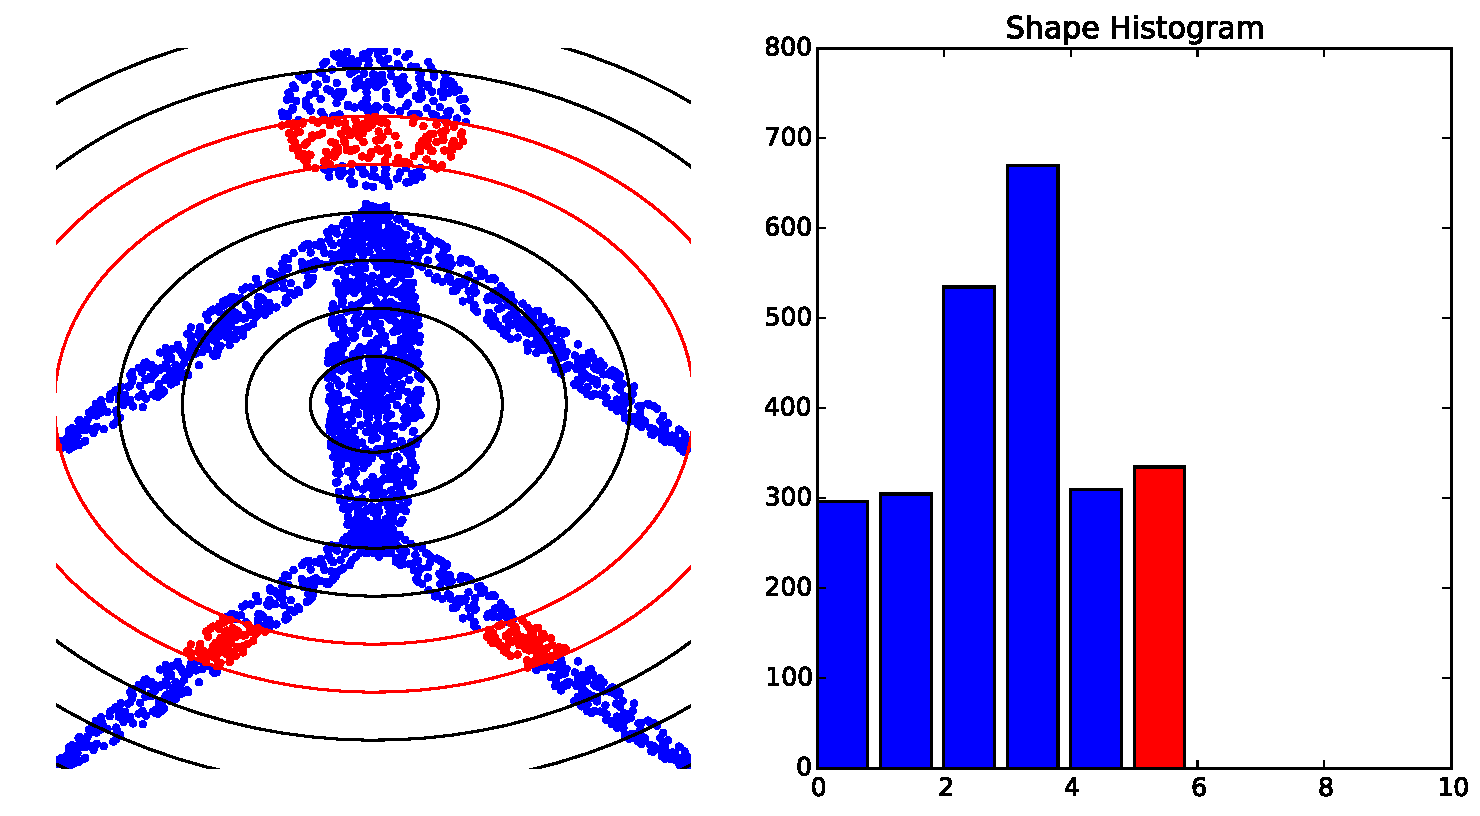
\includegraphics[width=\textwidth]{ShapeHist6.pdf}
\end{figure}

\end{frame}

\begin{frame}{Shape Histogram: Shells}

\begin{figure}[t]
	\centering
    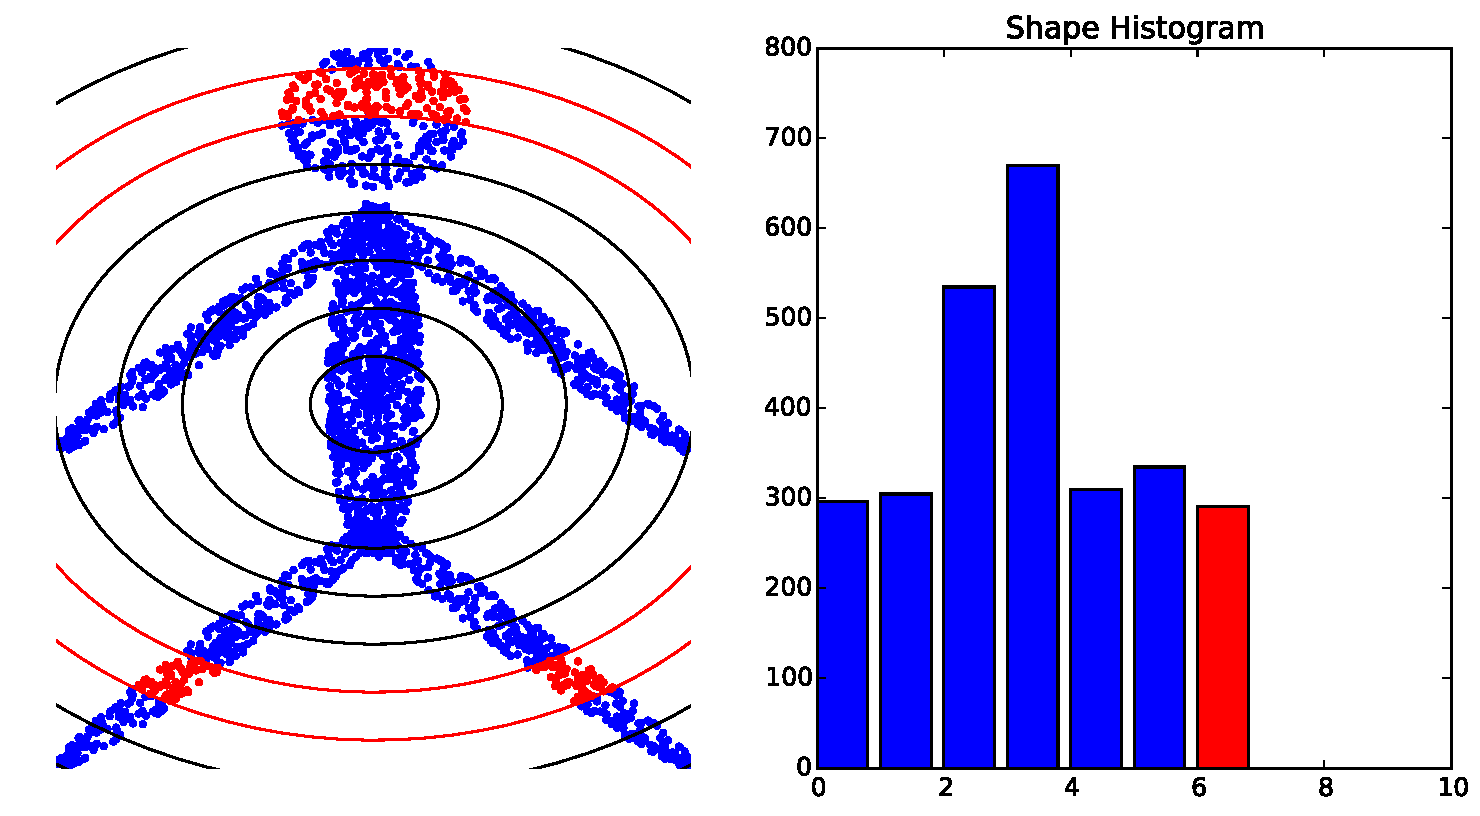
\includegraphics[width=\textwidth]{ShapeHist7.pdf}
\end{figure}

\end{frame}

\begin{frame}{Shape Histogram: Shells}

\begin{figure}[t]
	\centering
    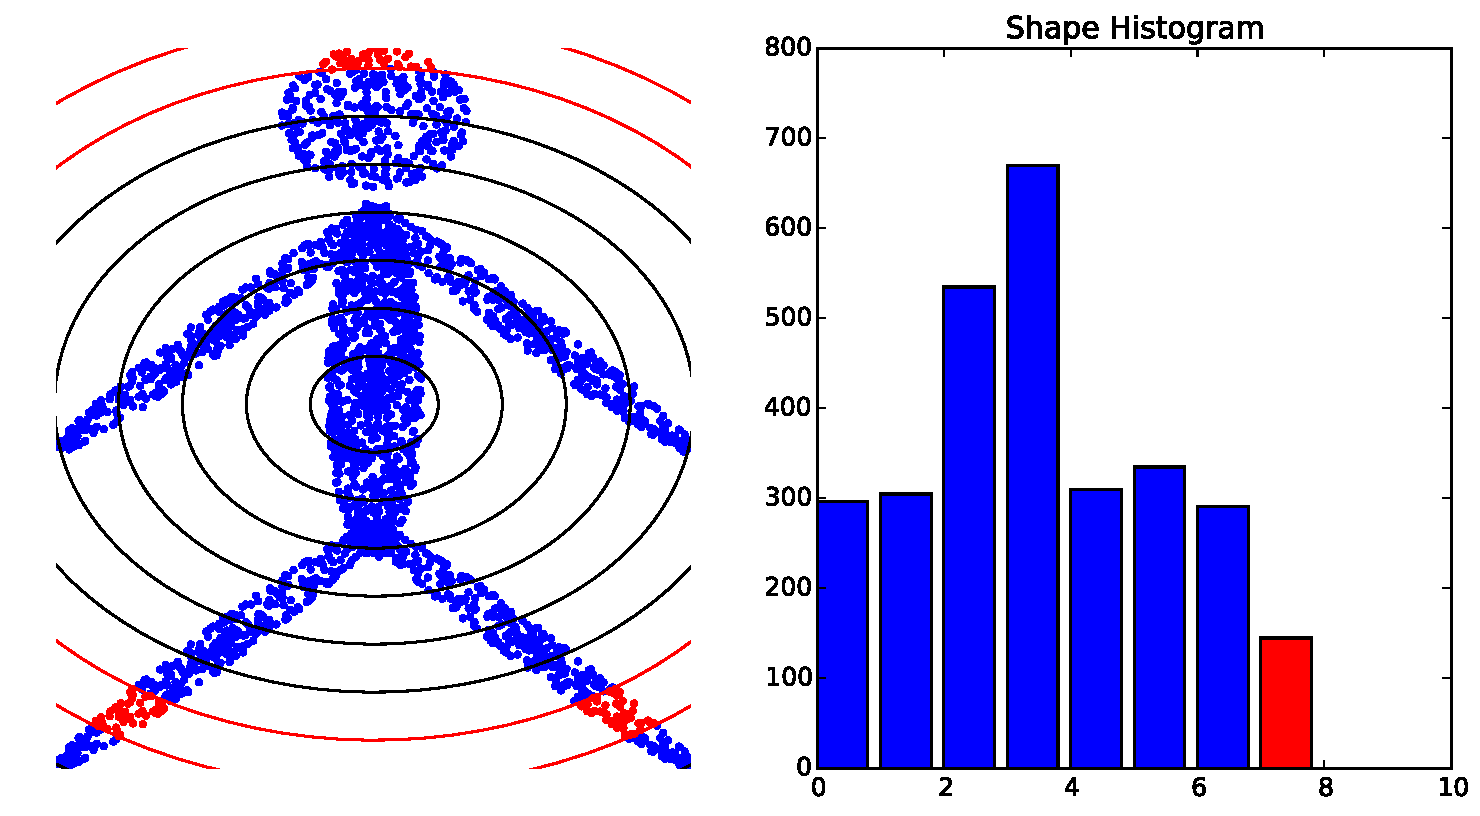
\includegraphics[width=\textwidth]{ShapeHist8.pdf}
\end{figure}

\end{frame}

\begin{frame}{Shape Histogram: Shells}

\begin{figure}[t]
	\centering
    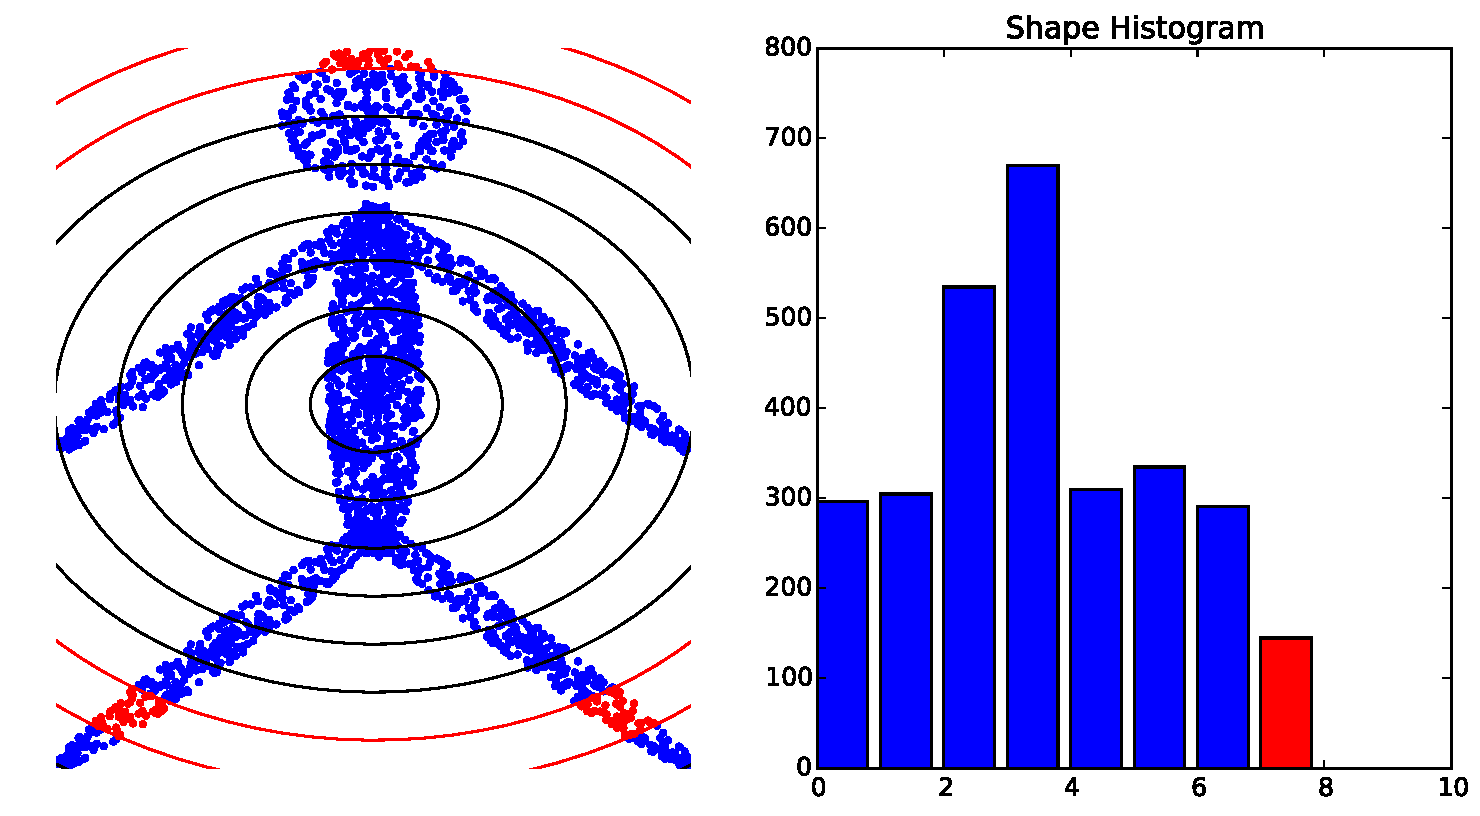
\includegraphics[width=0.7\textwidth]{ShapeHist8.pdf}
\end{figure}

\begin{itemize}[label=$\vartriangleright$]
\item \textcolor<2->{MidGreen}{Quick To Compute}
\uncover<3->{
\item \textcolor<4->{MidGreen}{Concise To Store}
}
\uncover<5->{
\item \textcolor<6->{MidGreen}{Rotation Invariant}
}
\uncover<7->{
\item \textcolor<8->{MidYellow}{Discerning}
}
\end{itemize}

\end{frame}

\begin{frame}{Shape Histogram: Shells}
What can't it tell apart?

SHOW VIDEO

\end{frame}

\begin{frame}{Shape Histogram: Shells And Sectors}

\begin{figure}[t]
	\centering
    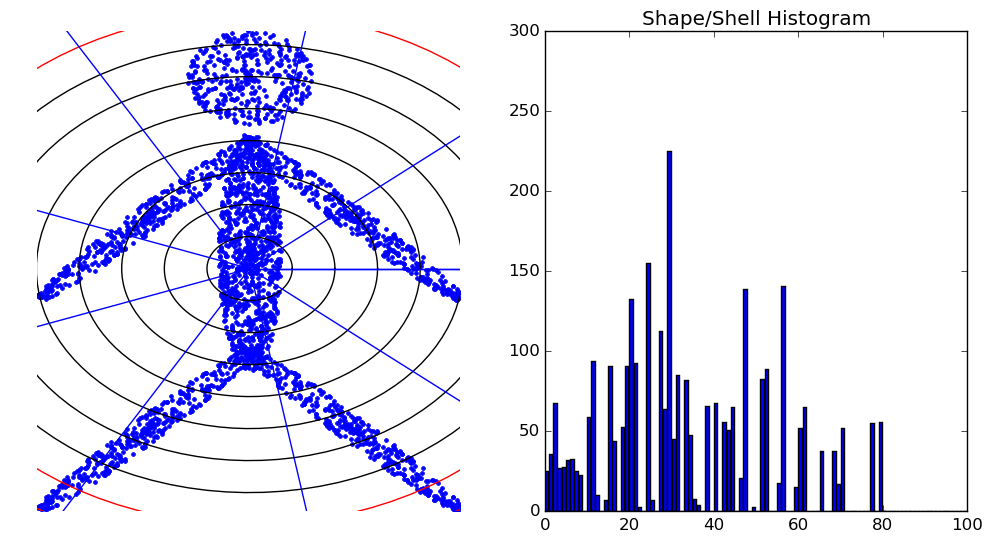
\includegraphics[width=\textwidth]{ShapeHistShellsSectors.png}
\end{figure}

SHOW VIDEO

\end{frame}

\begin{frame}{Shape Histogram: Shells And Sectors}

\begin{figure}[t]
	\centering
    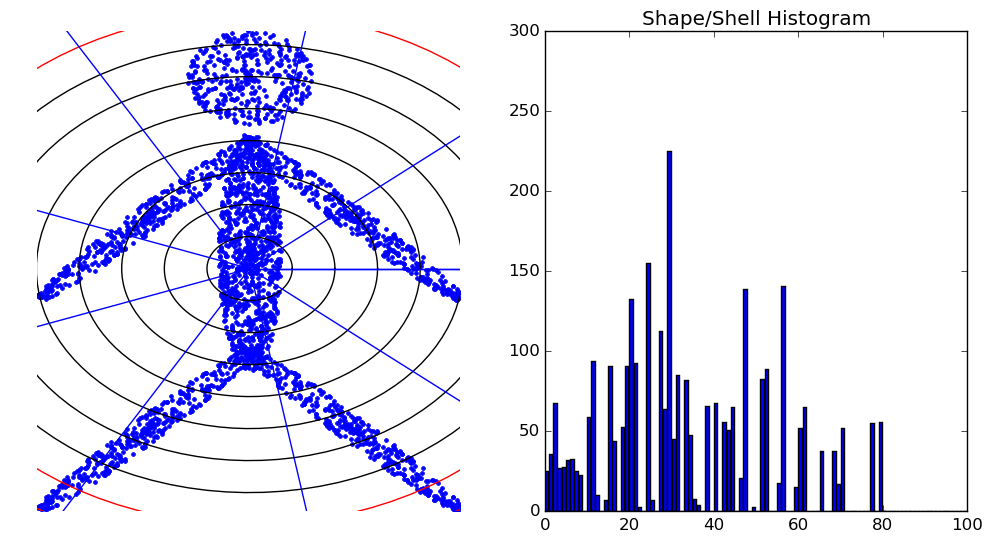
\includegraphics[width=\textwidth]{ShapeHistShellsSectors.png}
\end{figure}

Still Rotation Invariant?

\end{frame}


\begin{frame}{Shape Histogram: Shells And Sectors}

\begin{figure}[t]
	\centering
    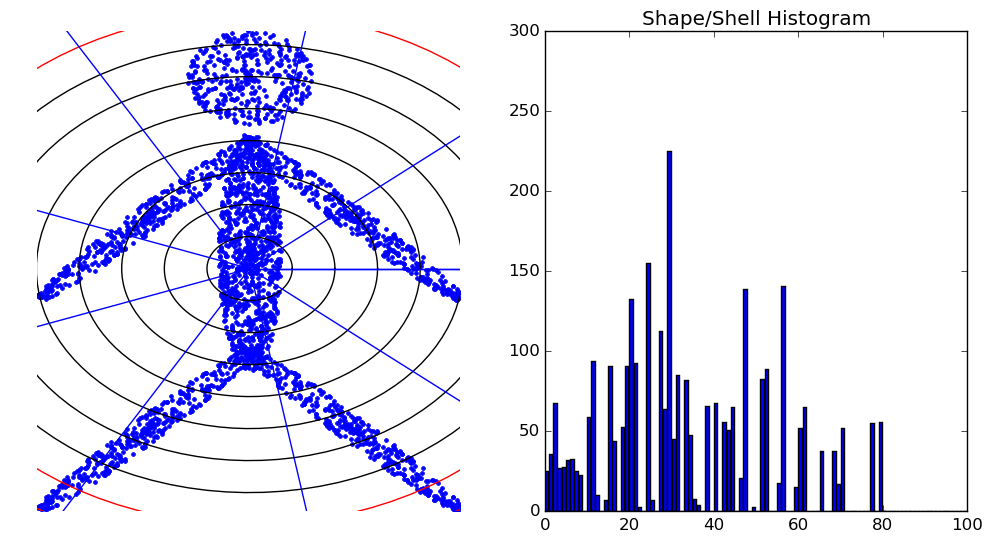
\includegraphics[width=\textwidth]{ShapeHistShellsSectors.png}
\end{figure}

\begin{itemize}[label=$\vartriangleright$]
\item Sort sectors within each shell
\item Record PCA {\em eigenvalues} within each shell
\end{itemize}

\end{frame}

\begin{frame}{Spin Images}

\begin{figure}[t]
	\centering
    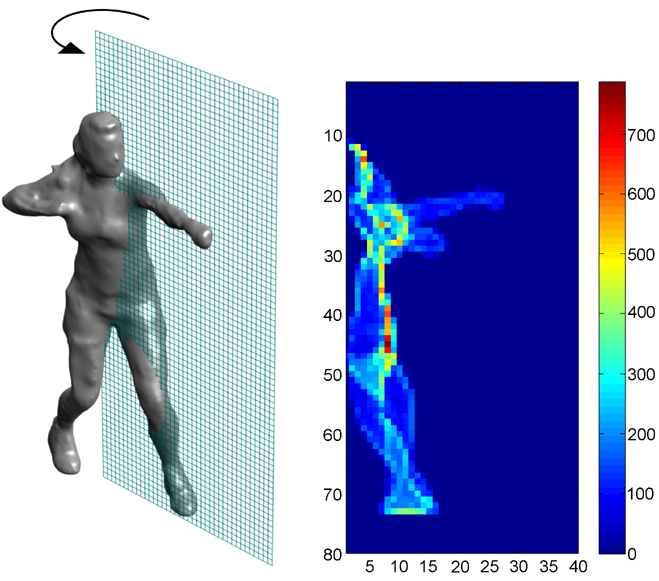
\includegraphics[width=0.7\textwidth]{SpinImage.png}
\end{figure}

\small Johnson/Herbert 1999, Figure Huang 2010

\end{frame}

\begin{frame}{Spin Images: Rubber Duck}

\begin{figure}[t]
	\centering
    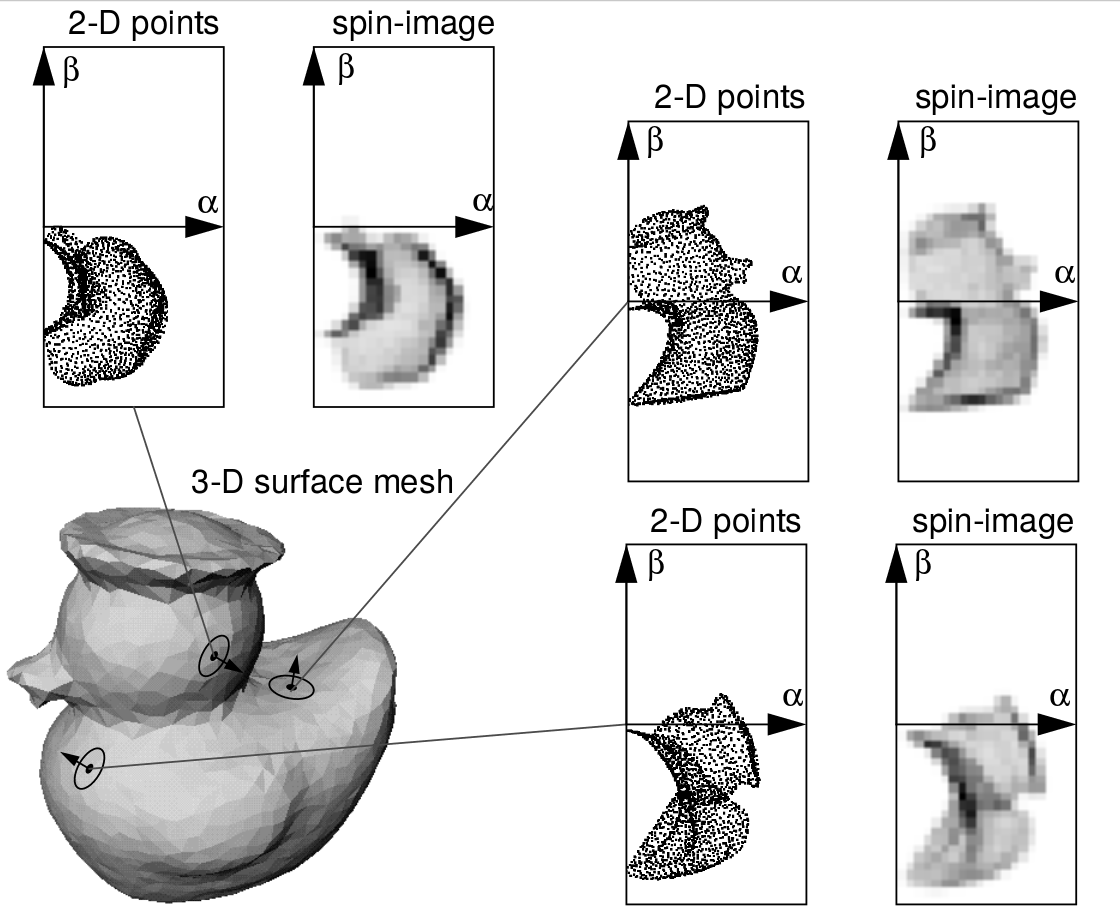
\includegraphics[width=0.7\textwidth]{RubberDuck_SpinImages.png}
\end{figure}

\small Johnson/Herbert 1999

\end{frame}


%\begin{frame}{Spin Images: Nearest Neighbor Binning}



%\end{frame}

%\begin{frame}{Spin Images: Bilinear Interpolation}


%\end{frame}

\begin{frame}{Spin Images}

\begin{figure}[t]
	\centering
    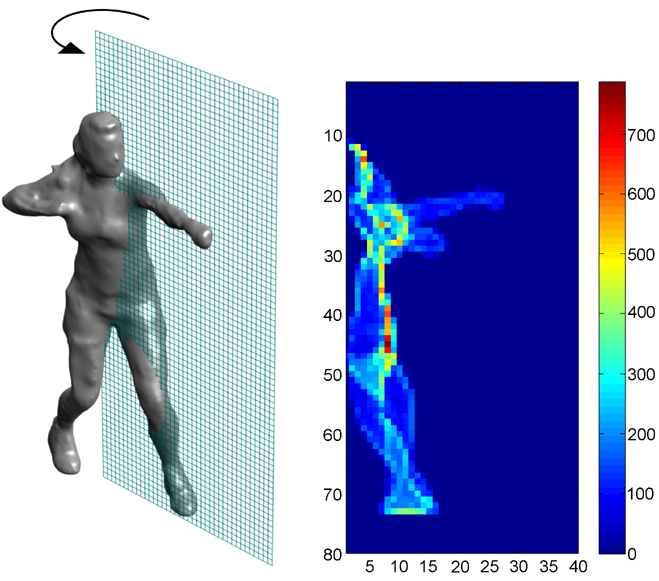
\includegraphics[width=0.5\textwidth]{SpinImage.png}
\end{figure}


\begin{itemize}[label=$\vartriangleright$]
\item \textcolor<2->{MidYellow}{Quick To Compute}
\uncover<3->{
\item \textcolor<4->{MidYellow}{Concise To Store} \uncover<4->{(Can compress images)}
}
\uncover<5->{
\item \textcolor<6->{MidGreen}{Rotation Invariant}
}
\uncover<6->{(Careful with principal axis stability)}
\uncover<7->{
\item \textcolor<8->{MidGreen}{Discerning}
}
\end{itemize}

\end{frame}

\begin{frame}{D2: Distance Histograms}

\begin{figure}[t]
	\centering
    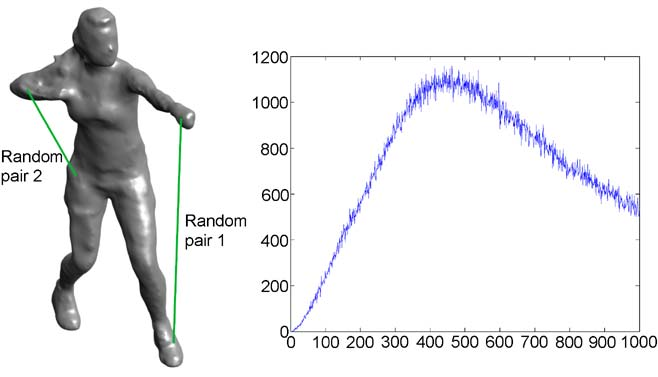
\includegraphics[width=\textwidth]{D2.png}
\end{figure}

\small Osada 2003, Figure from Huang 2010

\end{frame}


\begin{frame}{D2: Primitive Examples}

\begin{figure}[t]
	\centering
    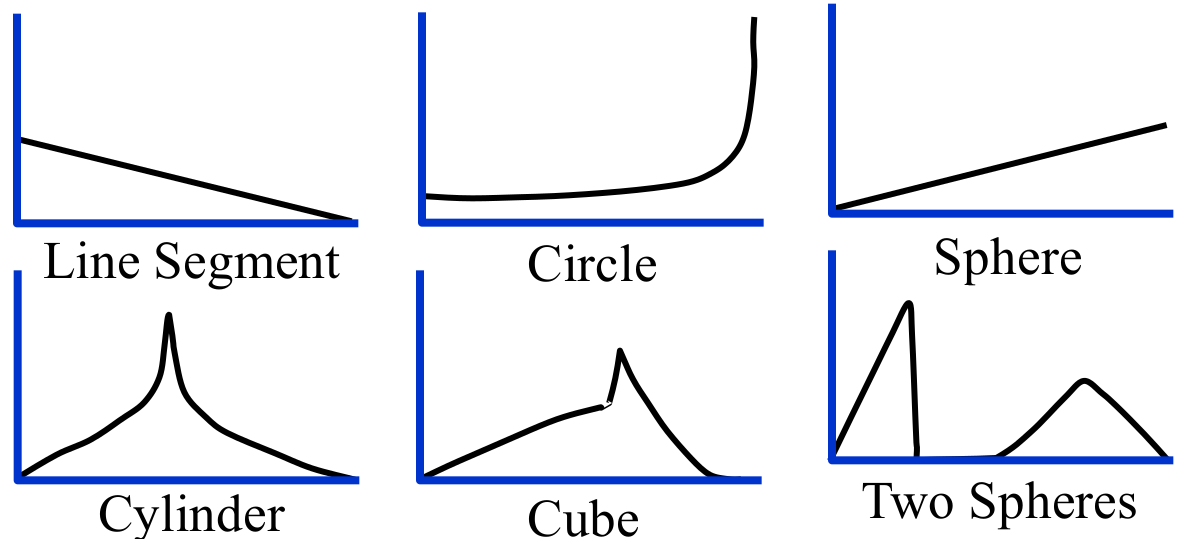
\includegraphics[width=\textwidth]{D2PrimitiveExamples.png}
\end{figure}

\small Osada 2003
\end{frame}

\begin{frame}{D2: Real Examples}

\begin{figure}[t]
	\centering
    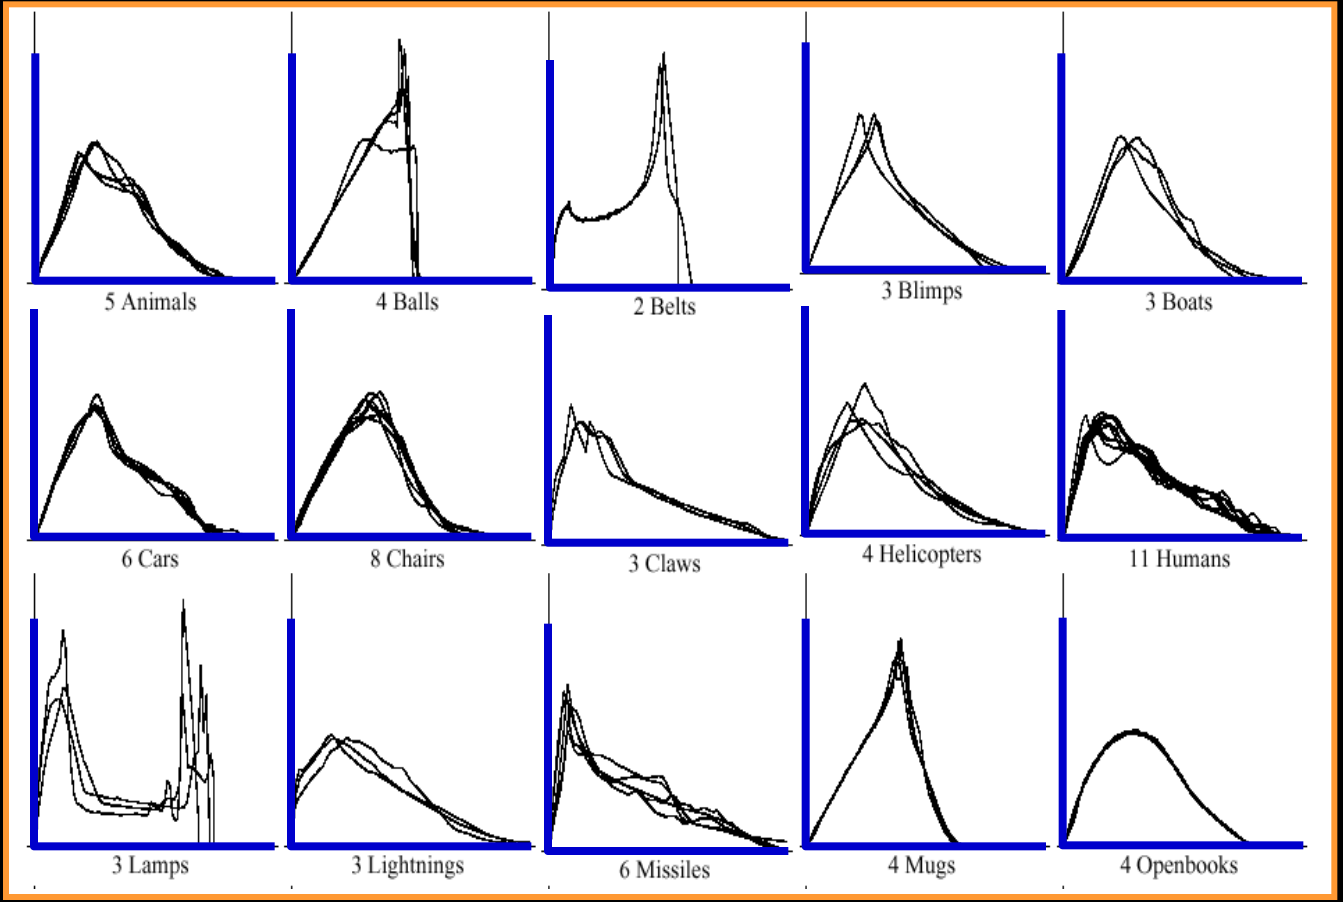
\includegraphics[width=\textwidth]{D2RealExamples.png}
\end{figure}

\small Osada 2003
\end{frame}

\begin{frame}{D1: Randomly Sample Points}

\begin{figure}[t]
	\centering
    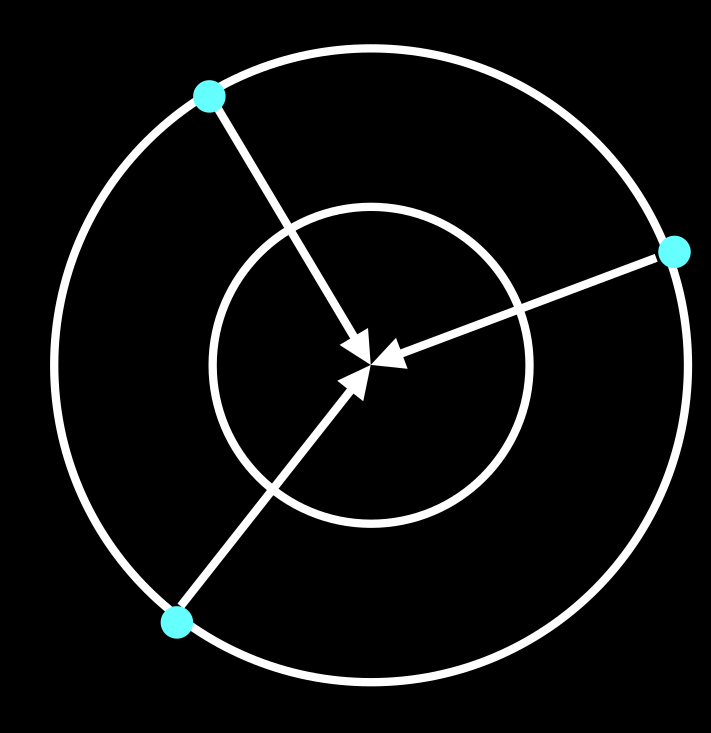
\includegraphics[width=0.6\textwidth]{D1.png}
\end{figure}

\small Osada 2003

\end{frame}

\begin{frame}{D3: Randomly Sample Areas}

\begin{figure}[t]
	\centering
    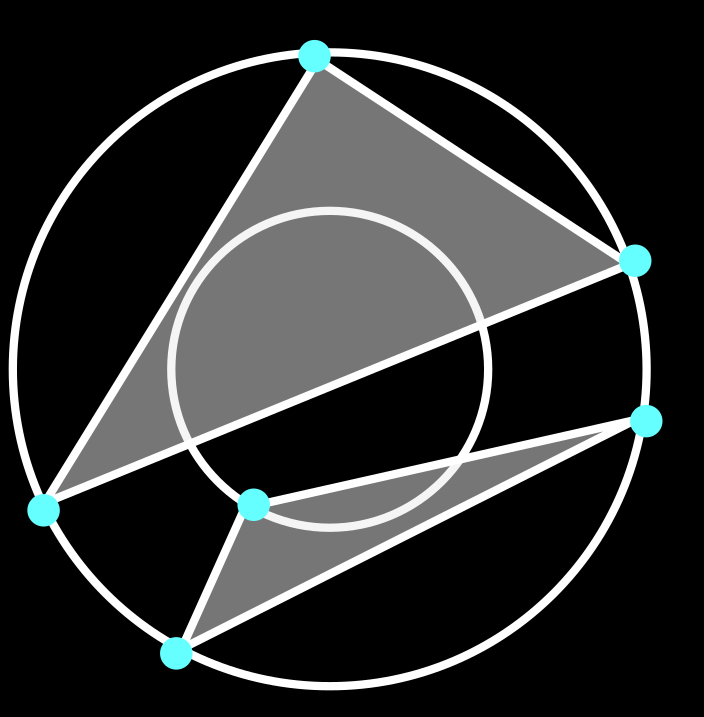
\includegraphics[width=0.6\textwidth]{D3.png}
\end{figure}

\small Osada 2003

\end{frame}

\begin{frame}{D4: Randomly Sample Volumes}

\begin{figure}[t]
	\centering
    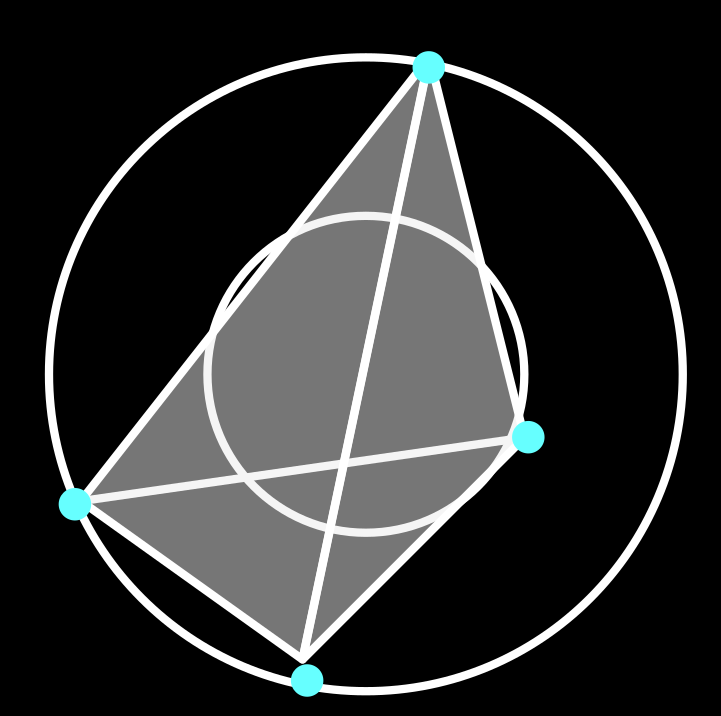
\includegraphics[width=0.6\textwidth]{D4.png}
\end{figure}

\small Osada 2003

\end{frame}

\begin{frame}{A3: Randomly Sample Angles}

\begin{figure}[t]
	\centering
    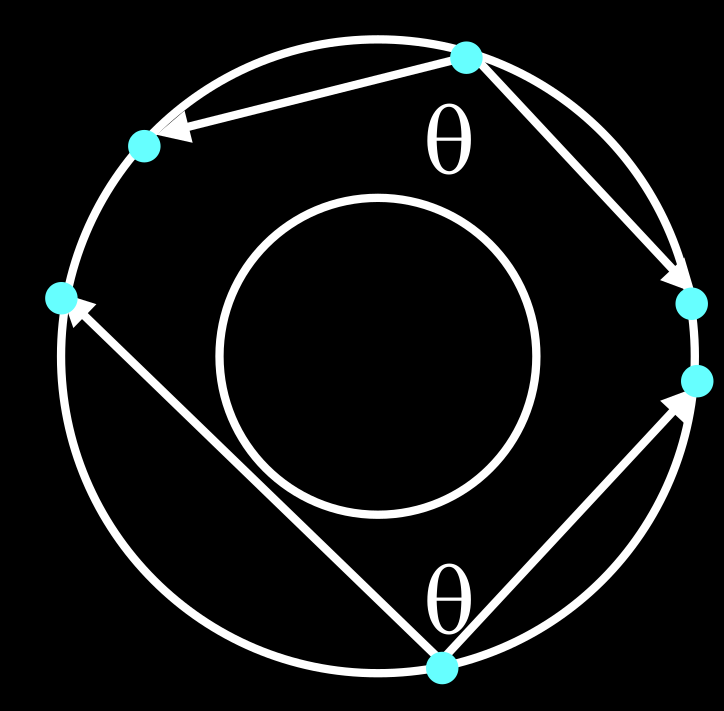
\includegraphics[width=0.6\textwidth]{A3.png}
\end{figure}

\small Osada 2003

\end{frame}

\begin{frame}{Extended Gaussian Image}

\begin{figure}[t]
	\centering
    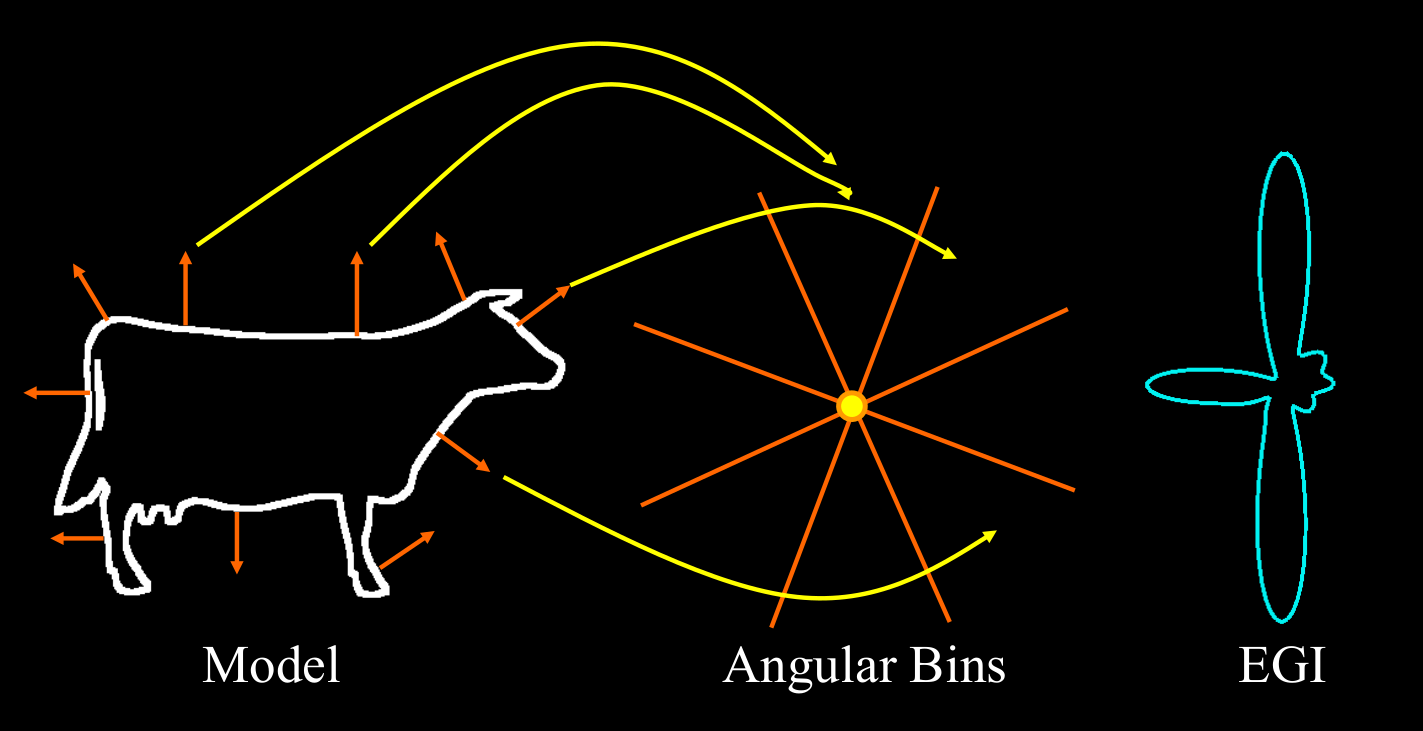
\includegraphics[width=\textwidth]{EGIOverview.png}
\end{figure}

\small Funkhouser 2004

\end{frame}

\begin{frame}{Extended Gaussian Image}

\begin{columns}[c]

\column{0.5\textwidth}
\begin{figure}[t]
    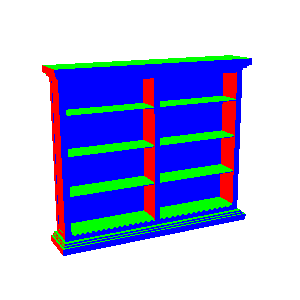
\includegraphics[width=\textwidth]{Bookcase.png}
\end{figure}

\column{0.5\textwidth}
\begin{figure}[t]
    
\includegraphics[width=\textwidth]{EGIBookcase.png}
\end{figure}

\end{columns}

\small Funkhouser 2004

\end{frame}


\begin{frame}{Extended Gaussian Image}

\begin{columns}[c]

\column{0.5\textwidth}
\begin{figure}[t]
    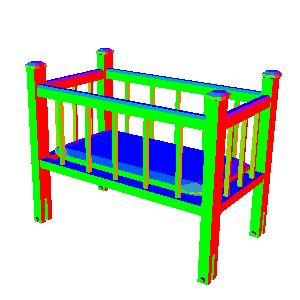
\includegraphics[width=\textwidth]{Crib.png}
\end{figure}

\column{0.5\textwidth}
\begin{figure}[t]
    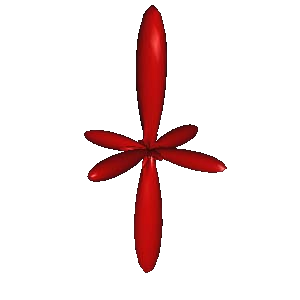
\includegraphics[width=\textwidth]{EGICrib.png}
\end{figure}

\end{columns}

\small Funkhouser 2004

\end{frame}


\begin{frame}{Extended Gaussian Image}

\begin{columns}[c]

\column{0.5\textwidth}
\begin{figure}[t]
    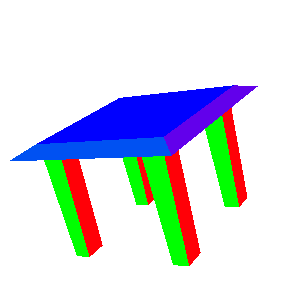
\includegraphics[width=\textwidth]{Table.png}
\end{figure}

\column{0.5\textwidth}
\begin{figure}[t]
    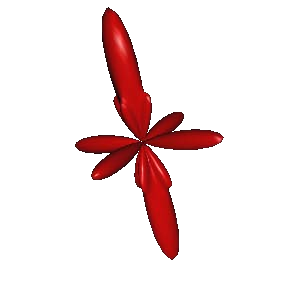
\includegraphics[width=\textwidth]{EGITable.png}
\end{figure}

\end{columns}



\begin{itemize}[label=$\vartriangleright$]

\uncover<2->{\item \textcolor<3->{MidGreen}{Efficient To Compute / Concise To Store}}

\end{itemize}

\small Funkhouser 2004

\end{frame}


\begin{frame}{Extended Gaussian Image}

\begin{columns}[c]

\column{0.5\textwidth}
\begin{figure}[t]
    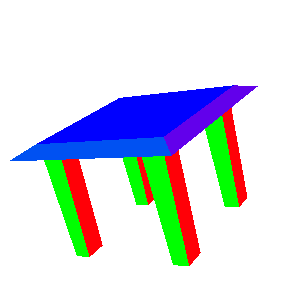
\includegraphics[width=\textwidth]{Table.png}
\end{figure}

\column{0.5\textwidth}
\begin{figure}[t]
    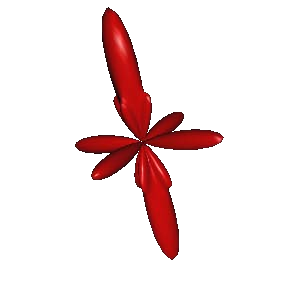
\includegraphics[width=\textwidth]{EGITable.png}
\end{figure}

\end{columns}



\begin{itemize}[label=$\vartriangleright$]

\uncover<1->{\item \textcolor<2->{MidYellow}{Discerning} \uncover<2->{(Only fully describes convex objects)} }

\end{itemize}

\small Funkhouser 2004

\end{frame}


\begin{frame}{Extended Gaussian Image}

\begin{columns}[c]

\column{0.5\textwidth}
\begin{figure}[t]
    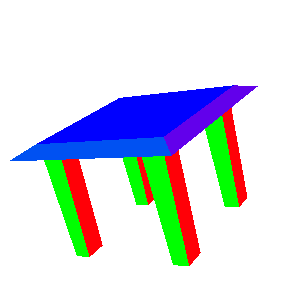
\includegraphics[width=\textwidth]{Table.png}
\end{figure}

\column{0.5\textwidth}
\begin{figure}[t]
    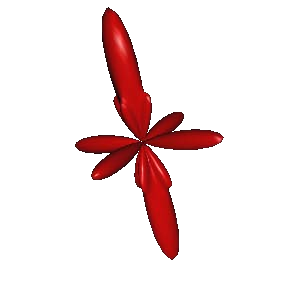
\includegraphics[width=\textwidth]{EGITable.png}
\end{figure}

\end{columns}


\begin{itemize}[label=$\vartriangleright$]

\uncover<1->{\item \textcolor<2->{red}{Rotation Invariant} \uncover<2->{(Rotate To Align With PCA Axes)} }

\end{itemize}

\small Funkhouser 2004

\end{frame}



\begin{frame}{Extended Gaussian Image}

\begin{columns}[c]

\column{0.5\textwidth}
\begin{figure}[t]
    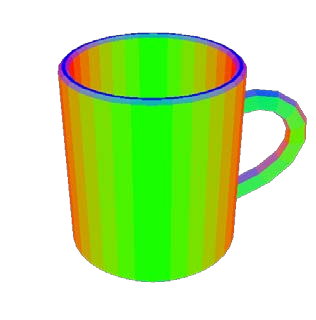
\includegraphics[width=0.5\textwidth]{origCoffeeMug.png}
\end{figure}

\column{0.5\textwidth}
\begin{figure}[t]
    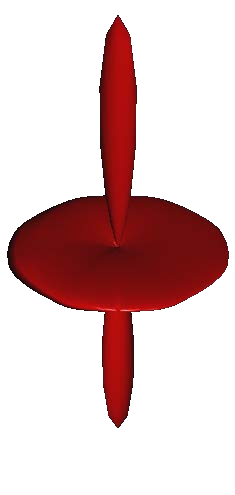
\includegraphics[width=0.5\textwidth]{EGIOrigCoffeeMug.png}
\end{figure}

\end{columns}

\begin{itemize}[label=$\vartriangleright$]

\item Robust To Noise?

\end{itemize}

\small Funkhouser 2004

\end{frame}


\begin{frame}{Extended Gaussian Image}

\begin{columns}[c]

\column{0.5\textwidth}
\begin{figure}[t]
    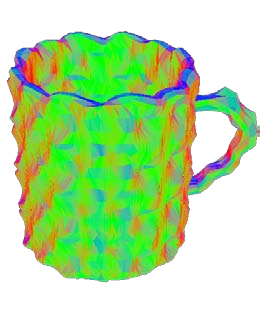
\includegraphics[width=0.5\textwidth]{NoiseCoffeeMug.png}
\end{figure}

\column{0.5\textwidth}
\begin{figure}[t]
    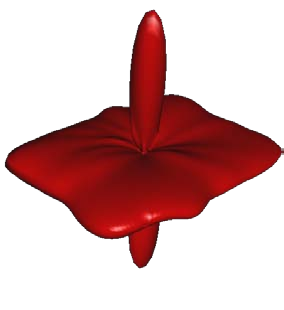
\includegraphics[width=0.5\textwidth]{EGINoiseCoffeeMug.png}
\end{figure}

\end{columns}

\begin{itemize}[label=$\vartriangleright$]

\item \textcolor{red}{Not Robust To Noise!}

\end{itemize}

\small Funkhouser 2004

\end{frame}


\begin{frame}{Table of Contents}
\begin{itemize}[label=$\vartriangleright$]
	\item Shape Statistics / Algorithms
\end{itemize}
\begin{itemize}[label=$\blacktriangleright$]
	\item Comparing Shape Statistics
\end{itemize}
\begin{itemize}[label=$\vartriangleright$]
	\item Classification / Performance Evaluation
\end{itemize}
\end{frame}


\begin{frame}{Normalize Histograms By Mass}


\[ h'[i] = \frac{h[i]}{\sum_{k=1}^N h[k]} \]

In other words, all bins should sum to 1

\end{frame}

\begin{frame}{Histogram Euclidean Distance}

For histograms $h_1$ and $h_2$

\[ d_E(h_1, h_2) = \sqrt{ \sum_{i=1}^N (h_1[i] - h_2[i])^2 } \]

Just thinking of $h_1$ and $h_2$ as high dimensional Euclidean vectors!  Each histogram bin is a dimension

\end{frame}

\begin{frame}{Histogram Cosine Distance}

\[ d_C(h_1, h_2) = \cos^{-1}\left(  \frac{ \vec{h_1} \cdot \vec{h_2} }{ ||\vec{h_1}|| ||\vec{h_2}|| } \right) \]

\end{frame}


\begin{frame}{Euclidean Distance Shortcomings}

\begin{figure}[t]
	\centering
    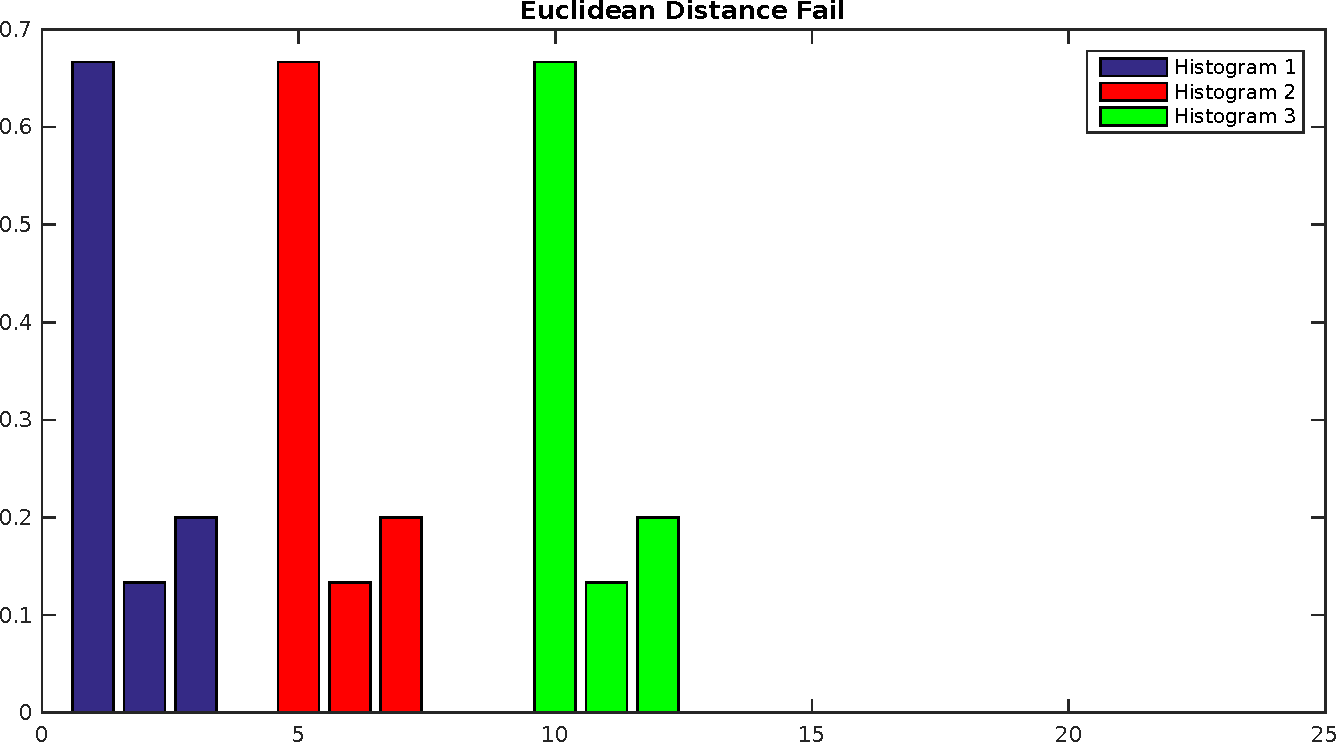
\includegraphics[width=\textwidth]{EuclidHistFail.pdf}
\end{figure}

They all have the same distance!

\end{frame}


\begin{frame}{Euclidean Distance Shortcomings}

\begin{figure}[t]
	\centering
    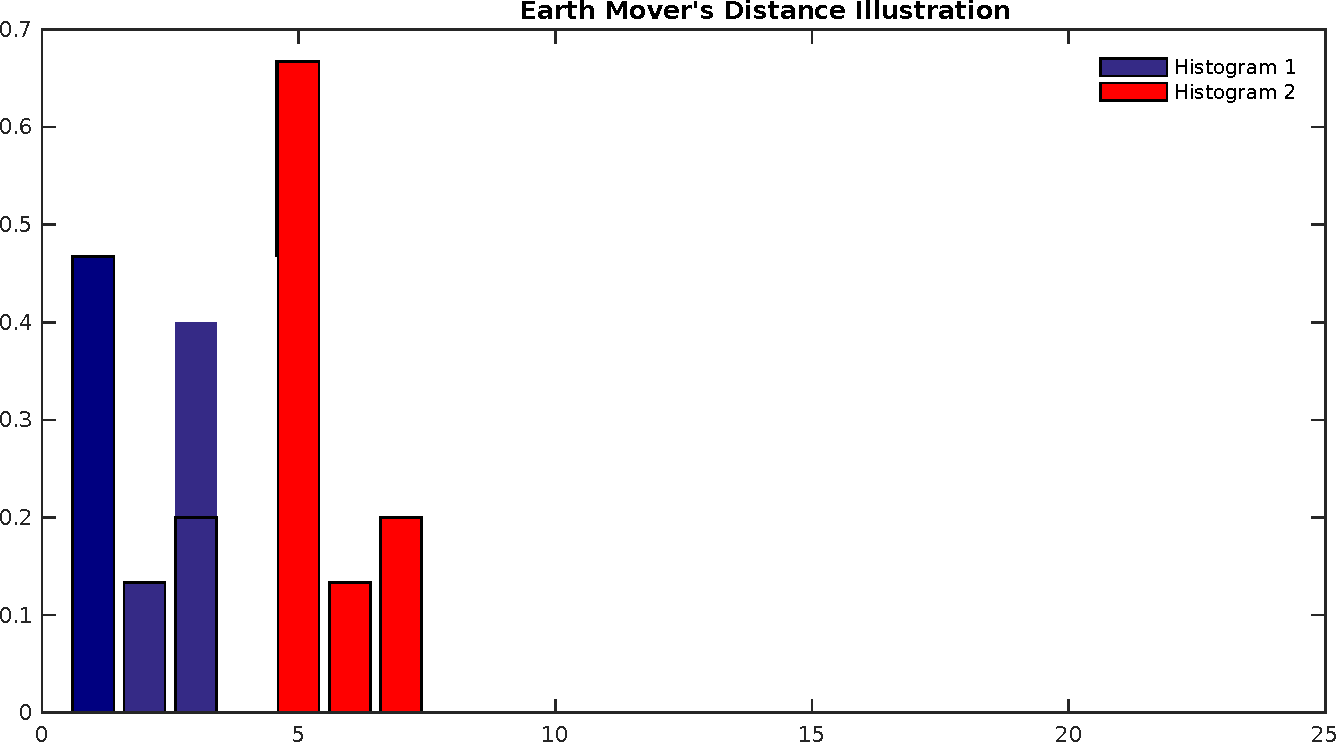
\includegraphics[width=\textwidth]{EMDVisual.pdf}
\end{figure}

Move earth from blue to red

\end{frame}

\begin{frame}{Earth Mover's Distance}

\begin{figure}[t]
	\centering
    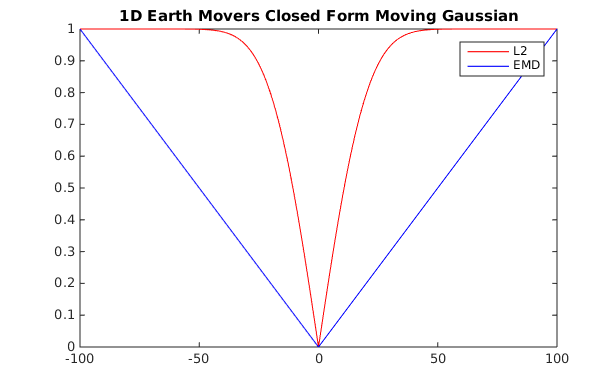
\includegraphics[width=0.8\textwidth]{1DEMDExample.png}
\end{figure}

\end{frame}

\begin{frame}{Chi Squared Distance}

\[ d_{\chi}(h_1, h_2) = \frac{1}{2} \sum_{i=1}^N \frac{(h_1[i] - h_2[i])^2}{h_1[i]+h_2[i]}\]

Exclude values for which $h_1[i] = h_2[i] = 0$

\end{frame}

\begin{frame}{Table of Contents}
\begin{itemize}[label=$\vartriangleright$]
	\item Shape Statistics / Algorithms
\end{itemize}
\begin{itemize}[label=$\vartriangleright$]
	\item Comparing Shape Statistics
\end{itemize}
\begin{itemize}[label=$\blacktriangleright$]
	\item Classification / Performance Evaluation
\end{itemize}
\end{frame}

\begin{frame}{Evaluation Strategy}

Do {\em leave one out} technique

\begin{itemize}

\item Use each item as test item in turn, compare to database

\end{itemize}

\begin{itemize}[label=$\blacktriangleright$]

\item Summarize evaluation statistics over entire database by {\em averaging them}

\end{itemize}

\end{frame}

\begin{frame}{Precision / Recall}

\begin{figure}[t]
	\centering
    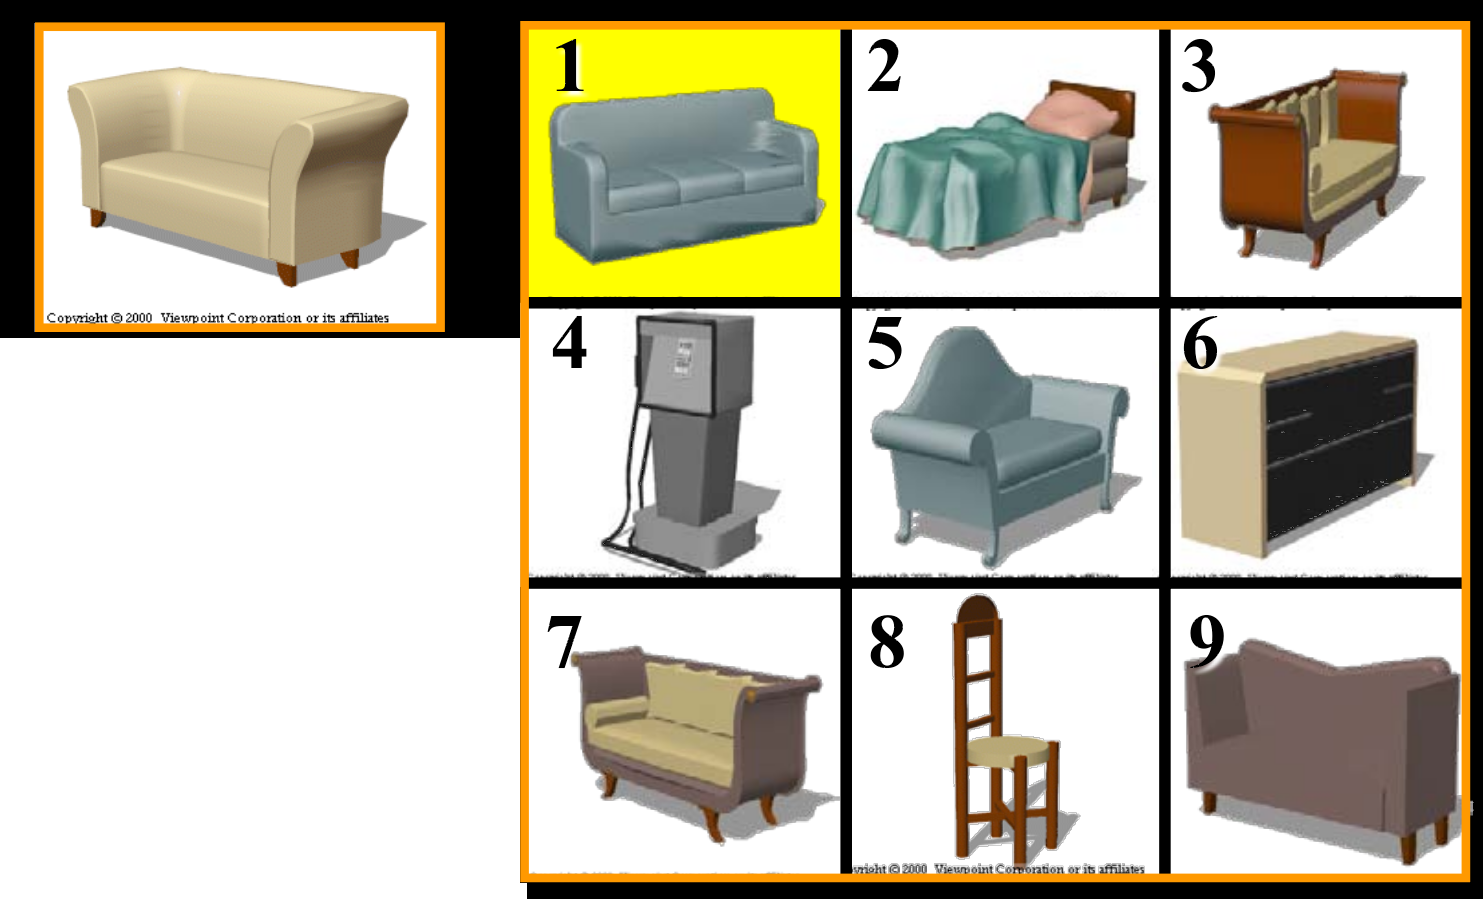
\includegraphics[width=\textwidth]{PrecisionRecall.png}
\end{figure}

Rusinkiewiz/Funkhouser 2009

\end{frame}

\begin{frame}{Other Evaluation Metrics}

\begin{itemize}[label=$\vartriangleright$]

\item Average Precision (Area Under Precision/Recall Curve)

\item Mean Reciprocal Rank (1/rank of first correct item)

\item Median Reciprocal Rank

\end{itemize}

1 is perfect score

\end{frame}


%\begin{frame}{Final Projects}
%Choices
%\begin{itemize}
%\item 1. Equidecomposing polygon meshes into each other in 3D, with SLERP animation
%\item 2. Ghissi Alterpiece: Real Time Rendering Effects for NC Museum of Art
%\item 3. Nasher Muesum Brummer Statue Heads Speech Transfer
%\item 4. MOCAP Data Animation in Browser / Skinning / 3D Lemur Tracking(?)
%\item 5. 3D Face Morphing
%\end{itemize}


%OR

%\begin{itemize}
%\item 6. Individual project with approval
%\end{itemize}

%\end{frame}

\end{document}

